%% REPLACE sXXXXXXX with your student number
\def\studentNumber{sXXXXXXX}


%% START of YOUR ANSWERS
%% Add answers to the questions below, by replacing the text inside the brackets {} for \youranswer{ "Text to be replaced with your answer." }. 
%
% Do not delete the commands for adding figures and tables. Instead fill in the missing values with your experiment results, and replace the images with your own respective figures.
%
% You can generally delete the placeholder text, such as for example the text "Question Figure 2 - Replace the images ..." 
%
% There are 18 TEXT QUESTIONS (a few of the short first ones have their answers added to both the Introduction and the Abstract). Replace the text inside the brackets of the command \youranswer with your answer to the question.
%
% There are also 3 "questions" to replace some placeholder FIGURES with your own, and 3 "questions" asking you to fill in the missing entries in the TABLES provided. 
%
% NOTE! that questions are ordered by the order of appearance of their answers in the text, and not by the order you should tackle them. Specifically, you cannot answer Questions 2, 3, and 4 before concluding all of the relevant experiments and analysis. Similarly, you should fill in the TABLES and FIGURES before discussing the results presented there. 
%
% NOTE! If for some reason you do not manage to produce results for some FIGURES and TABLES, then you can get partial marks by discussing your expectations of the results in the relevant TEXT QUESTIONS (for example Question 8 makes use of Table 1 and Figure 2).
%
% Please refer to the coursework specification for more details.


%% - - - - - - - - - - - - TEXT QUESTIONS - - - - - - - - - - - - 

%% Question 1:
\newcommand{\questionOne} {
\youranswer{Question 1 - Summarise why overfitting is a problem}
}

%% Question 2:
\newcommand{\questionTwo} {
\youranswer{Question 2 - Summarise the effect increasing width and depth of the architecture had on overfitting}
}

%% Question 3:
\newcommand{\questionThree} {
\youranswer{Question 3 - Summarise what your results show you about the effect of the tested approaches on overfitting and the performance of the trained model}
}

%% Question 4:
\newcommand{\questionFour} {
\youranswer{Question 4 - Give your overall conclusions}
}

%% Question 5:
\newcommand{\questionFive} {
\youranswer{Question 5 - Explain in detail, and in your own words, why overfitting is a problem}
}

%% Question 6:
\newcommand{\questionSix} {
\youranswer{Question 6 - Explain the relevance of "network capacity" to overfitting}
}

%% Question 7:
\newcommand{\questionSeven} {
\youranswer{Question 7 - Explain what these figures contain and how the curves evolve, and spot where overfitting occurs. Reason based on the min/max points and velocities (direction and magnitude of change) of the accuracy and error curves}
}

%% Question 8:
\newcommand{\questionEight} {
\youranswer{Question 8 - Explain your network width experiment results by using the relevant figure and table}
}

%% Question 9:
\newcommand{\questionNine} {
\youranswer{Question 9 - Discuss whether varying width affects the results in a consistent way, and whether the results are expected and match well with the prior knowledge (by which we mean your expectations as are formed from the relevant Theory and literature)}
}

%% Question 10:
\newcommand{\questionTen} {
\youranswer{Question 10 - Explain your network depth experiment results by using the relevant figure and table}
}

%% Question 11:
\newcommand{\questionEleven} {
\youranswer{Question 11 - Discuss whether varying depth affects the results in a consistent way, and whether the results are expected and match well with the prior knowledge (by which we mean your expectations as are formed from the relevant Theory and literature)}
}

%% Question 12:
\newcommand{\questionTwelve} {
\youranswer{Question 12 - Compare and discuss how varying width and height changes the performance and overfitting in your experiments}
}

%% Question 13:
\newcommand{\questionThirteen} {
\youranswer{Question 13 - Explain how one could use a combination of L1 and L2 regularization. Discuss any potential benefits of this approach}
}

%% Question 14:
\newcommand{\questionFourteen} {
\youranswer{Question 14 - Explain the experimental details (e.g. hyperparameters), discuss the results in terms of their generalization performance and overfitting. Select and test the best performing model as part of this analysis}
}

%% Question 15:
\newcommand{\questionFifteen} {
\youranswer{Question 15 - Assume you were able to run 8 further experiments where you could combine Dropout and L1, and/or Dropout and L2 regularization. Which 8 runs would you pick and what question(s) would you aim to answer? Make sure you define the experiment setup, including any relevant hyperparameters}
}

%% Question 16:
\newcommand{\questionSixteen} {
\youranswer{Question 16 - Explain, in your own words, why the equivalence between L2 weight penalty and weight decay in Adam optimizer requires a more complex relation; a preconditioner matrix $\bm{M}_t$ rather than a scalar relation}
}

%% Question 17:
\newcommand{\questionSeventeen} {
\youranswer{Question 17 - Based on \textbf{Algorithm 2} in \cite{loshchilov2019decoupled}, discuss whether your code with L2 Weight Penalty in the MLP library implements ``Adam with L2 regularization'', ``Adam with decoupled weight decay (AdamW)'' or another variation. Refer to the MLP code, pointing to the specific files and functions to justify your answer}
}

%% Question 18:
\newcommand{\questionEighteen} {
\youranswer{Question 18 - Briefly draw your conclusions based on the results from the previous sections (what are the take-away messages?) and conclude your report with a recommendation for future directions}
}

%% - - - - - - - - - - - - FIGURES - - - - - - - - - - - - 

%% Question Figure 2:
\newcommand{\questionFigureTwo} {
\youranswer{Question Figure 2 - Replace the images in Figure 2 with figures depicting the accuracy and error, training and validation curves for your experiments varying the number of hidden units.
%
\begin{figure}[t]
    \centering
    \begin{subfigure}{\linewidth}
        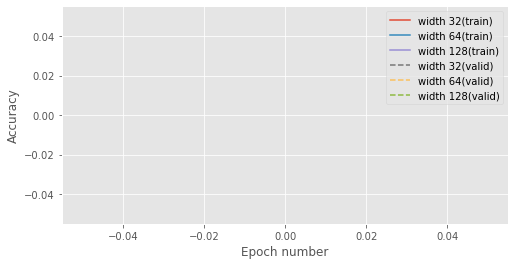
\includegraphics[width=\linewidth]{figures/empty_acc_curve_width.png}
        \caption{accuracy by epoch}
        \label{fig:width_acccurves}
    \end{subfigure} 
    \begin{subfigure}{\linewidth}
        \centering
        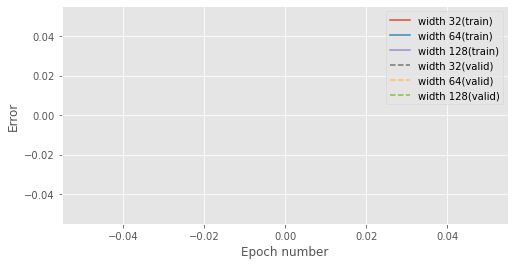
\includegraphics[width=\linewidth]{figures/empty_error_curve_width.png}
        \caption{error by epoch}
        \label{fig:width_errorcurves}
    \end{subfigure} 
    \caption{Training and validation curves in terms of classification accuracy (a) and cross-entropy error (b) on the EMNIST dataset for different network widths.}
    \label{fig:width}
\end{figure} 
}
}

%% Question Figure 3:
\newcommand{\questionFigureThree} {
\youranswer{Question Figure 3 - Replace these images with figures depicting the accuracy and error, training and validation curves for your experiments varying the number of hidden layers.
%
\begin{figure}[t]
    \centering
    \begin{subfigure}{\linewidth}
        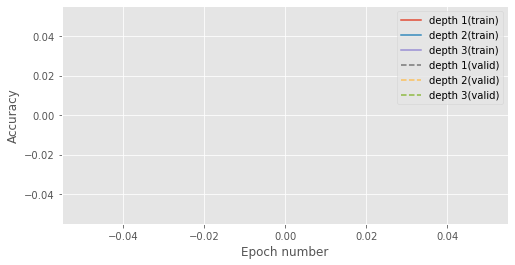
\includegraphics[width=\linewidth]{figures/empty_acc_curve_depth.png}
        \caption{accuracy by epoch}
        \label{fig:depth_acccurves}
    \end{subfigure} 
    \begin{subfigure}{\linewidth}
        \centering
        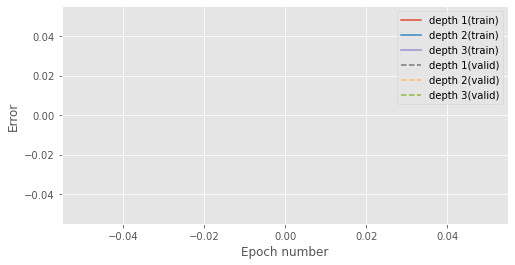
\includegraphics[width=\linewidth]{figures/empty_error_curve_depth.png}
        \caption{error by epoch}
        \label{fig:depth_errorcurves}
    \end{subfigure} 
    \caption{Training and validation curves in terms of classification accuracy (a) and cross-entropy error (b) on the EMNIST dataset for different network depths.}
    \label{fig:depth}
\end{figure} 
}
}

%% Question Figure 4:
\newcommand{\questionFigureFour} {
\youranswer{Question Figure 4 - Replace these images with figures depicting the Validation Accuracy and Generalisation Gap (difference between validation and training error) for each of the experiment results varying the Dropout inclusion rate, and L1/L2 weight penalty depicted in Figure 3 (including any results you have filled in).
%
\begin{figure*}[t]
    \centering
    \begin{subfigure}{.475\linewidth}
        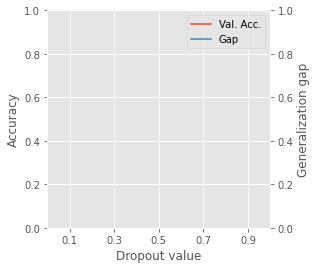
\includegraphics[width=\linewidth]{figures/empty_dropout_plot.png}
        \caption{Accuracy and error by inclusion probability.}
        \label{fig:dropoutrates}
    \end{subfigure} 
    \begin{subfigure}{.475\linewidth}
        \centering
        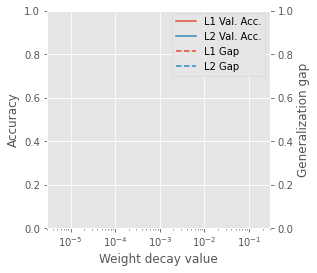
\includegraphics[width=\linewidth]{figures/empty_wd_plot.png}
        \caption{Accuracy and error by weight penalty.}
        \label{fig:weightrates}
    \end{subfigure} 
    \caption{Accuracy and error by regularization strength of each method (Dropout and L1/L2 Regularization).}
    \label{fig:hp_search}
\end{figure*}
}
}

%% - - - - - - - - - - - - TABLES - - - - - - - - - - - - 

%% Question Table 1:
\newcommand{\questionTableOne} {
\youranswer{
Question Table 1 - Fill in Table 1 with the results from your experiments varying the number of hidden units.
%
\begin{table}[t]
    \centering
    \begin{tabular}{c|ccc}
    \toprule
        \# Hidden Units & Val. Acc. & Train Error & Val. Error\\
    \midrule
         32            &    --.-   &  -.--- &   -.---            \\
         64            &    --.-   &  -.---  &   -.---               \\
         128           &    --.-   &  -.---  &   -.---           \\ 
    \bottomrule
    \end{tabular}
    \caption{Validation accuracy (\%) and training/validation error (in terms of cross-entropy error) for varying network widths on the EMNIST dataset.}
    \label{tab:width_exp}
\end{table}
}
}

%% Question Table 2:
\newcommand{\questionTableTwo} {
\youranswer{
Question Table 2 - Fill in Table 2 with the results from your experiments varying the number of hidden layers.
%
\begin{table}[t]
    \centering
    \begin{tabular}{c|ccc}
    \toprule
        \# Hidden Layers & Val. Acc. & Train Error & Val. Error \\
    \midrule
         1               &      --.-      &   -.--- & -.---                \\
         2               &    --.-       &  -.--- & -.---                 \\
         3               &      --.-      &   -.--- & -.---                \\ 
    \bottomrule
    \end{tabular}
    \caption{Validation accuracy (\%) and training/validation error (in terms of cross-entropy error) for varying network depths on the EMNIST dataset.}
    \label{tab:depth_exps}
\end{table}
}
}

%% Question Table 3:
\newcommand{\questionTableThree} {
\youranswer{
Question Table 3 - Fill in Table 3 with the results from your experiments for the missing hyperparameter values for each of L1 regularisation, L2 regularisation, and Dropout (use the values shown on the table).
%
\begin{table*}[t]
    \centering
    \begin{tabular}{c|c|ccc}
    \toprule
        Model    &  Hyperparameter value(s) & Validation accuracy & Train Error & Validation Error \\
    \midrule
    \midrule
        Baseline &  -                    &               0.837 &       0.241 &  0.533          \\
    \midrule
        \multirow{4}*{Dropout}
                 & 0.6                   &  80.7                &      0.549 & 0.593     \\
                 & 0.7 & --.- & -.--- & -.---  \\
                 & 0.85 & 85.1 &  0.329 &  0.434 \\
                 & 0.97 & 85.4 &  0.244 & 0.457  \\
    \midrule
        \multirow{4}*{L1 penalty}
                 & 5e-4 & 79.5 & 0.642 & 0.658 \\
                 & 1e-3 & --.- & -.--- & -.--- \\
                 & 5e-3 & 2.41 & 3.850 & 3.850 \\
                 & 5e-2 & 2.20 & 3.850 & 3.850 \\
    \midrule
        \multirow{4}*{L2 penalty}  
                 & 5e-4 & 85.1 & 0.306 & 0.460 \\
                 & 1e-3 & --.- & -.--- & -.--- \\
                 & 5e-3 & 81.3 & 0.586 & 0.607 \\
                 & 5e-2 & 39.2 & 2.258 & 2.256  \\      
    \bottomrule
    \end{tabular}
    \caption{Results of all hyperparameter search experiments. \emph{italics} indicate the best results per series (Dropout, L1 Regularization, L2 Regularization) and \textbf{bold} indicates the best overall.}
    \label{tab:hp_search}
\end{table*}
}
}

%% END of YOUR ANSWERS